%%%%%%%%%%%%%%%%%%%%%%%%%%%%%%%%%%%% Chapter Template

\chapter{Solução} 	% Main chapter title Conceção e Implementação
\label{Chapter3} 		% For referencing the chapter elsewhere, 


\noindent Este capítulo apresenta a solução desenvolvida para o problema descrito no Capítulo~\ref{Chapter2}, começa por enquadrar as ferramentas e tecnologias escolhidas, seguindo-se da descrição da arquitetura do sistema, do modelo de dados e, por último, da implementação das componentes de \textit{front-end} e de \textit{back-end}.

\section{Ferramentas e Tecnologias}
\label{sec:Ch3.1}

\noindent A escolha desta tecnologia é referenciada também pela literatura, que evidência vantagens relativamente a alternativas mais antigas, como o \textit{AWT} e o \textit{Swing}, nomeadamente ao nível da separação entre a definição visual, feita em \textit{FXML}, e a lógica da aplicação~\cite{Pereira2020}. A construção dos ecrãs recorre ao \textit{Scene Builder}, uma ferramenta visual de edição de \textit{FXML}  documentada~\cite{Vivien2010}.


\noindent Do lado do servidor, é utilizado o \textit{Apache Tomcat}, responsável por expor uma \ac{api} \ac{rest} que serve de interface entre o cliente gráfico e a base de dados. A comunicação entre as duas camadas é efetuada sobre \ac{http}, recorrendo ao formato \ac{json} para a troca de mensagens, por ser um formato leve e nativamente suportado pelas bibliotecas \textit{Java}.

\noindent A persistência dos dados em \ac{sgbd} \textit{MySQL}, acedida a partir do \textit{back-end} através de \ac{jdbc}, a interface padrão do \textit{Java} para ligação a bases de dados relacionais. O desenvolvimento é realizado sobre o \ac{jdk}, com recurso a um \ac{ide} para a edição e depuração do código, e ao \textit{Git}, por forma a documentar a evolução do projeto ao longo das cinco semanas definidas no planeamento (Tabela~\ref{tab:cronograma}).

Para justificar a origem das bibliotecas gráficas utilizadas e assegurar a reprodutibilidade do ambiente de desenvolvimento, foi documentado o processo de obtenção do respetivo SDK através do distribuidor oficial, conforme ilustra a Figura~\ref{fig:instalacao_javafx}.

\begin{figure}[htbp]
    \centering
    \includegraphics[width=0.85\textwidth]{InstalacaoJavaFX.png}
    \caption{Página de download do JavaFX SDK disponibilizado pela Gluon.}
    \label{fig:instalacao_javafx}
\end{figure}

Tal como referido anteriormente, a desassociação do JavaFX do JDK base a partir da versão 11 exige a configuração explícita de argumentos de execução e do caminho dos módulos. A ausência do parâmetro \texttt{--module-path} resulta no erro de compilação e execução evidenciado na Figura~\ref{fig:erro_modular_javafx}.

\begin{figure}[htbp]
    \centering
    \includegraphics[width=0.85\textwidth]{JavaFXdeixoudevirincluídonoJDK.png}
    \caption{Erro de execução decorrente da falta de configuração do \texttt{--module-path}.}
    \label{fig:erro_modular_javafx}
\end{figure}

Após a correta parametrização das variáveis de ambiente e bibliotecas modulares, desenvolveu-se uma prova de conceito básica para validar o ciclo de vida da aplicação gráfica e a correta renderização na máquina de desenvolvimento (Figura~\ref{fig:hello_javafx}).

\begin{figure}[htbp]
    \centering
    \includegraphics[width=0.90\textwidth]{HelloJavaFxTeste1.png}
    \caption{Janela de teste inicial ("Olá, JavaFX!") validando o ambiente gráfico.}
    \label{fig:hello_javafx}
\end{figure}

\section{Arquitetura}
\label{sec:Ch3.2}


\noindent A aplicação segue uma arquitetura distribuída de três camadas, tal como definido nos objetivos do trabalho: apresentação, lógica de negócio e dados. A Figura~\ref{fig:arquitetura} ilustra esta organização e o protocolo de comunicação utilizado entre cada camada.


\begin{figure}[htbp]
    \centering
    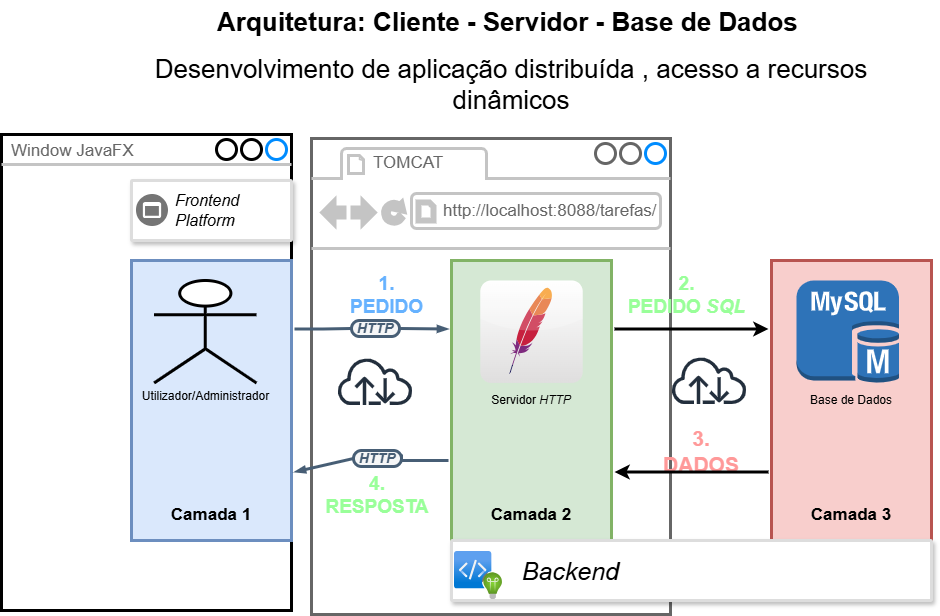
\includegraphics[scale=0.30]{figures/Diagrama-3-camada.drawio}
    \caption{Arquitetura distribuída de três camadas da aplicação \textit{Gestão de Tarefas}.}
    \label{fig:arquitetura}
\end{figure}

\noindent Como representado na Figura~\ref{fig:arquitetura}, o cliente \textit{JavaFX} não acede diretamente à base de dados, comunicando exclusivamente com o servidor \textit{Tomcat} através de pedidos \ac{http}.  O servidor, por sua vez, está na camada intermédia, com acesso à camada de dados, que comunica  com o \ac{sgbd} \textit{MySQL} através de \ac{jdbc}. 

\section{Modelo de Dados}
\label{sec:Ch3.3}

\noindent O modelo de dados da aplicação assenta em duas entidades principais: \textit{Utilizador} e \textit{Tarefa}, relacionadas entre si numa associação de um para muitos, já que um utilizador pode ser responsável por várias tarefas, mas cada tarefa pertence apenas a um utilizador. A Figura~\ref{fig:ermodel} apresenta o modelo relacional simplificado destas duas entidades.


\begin{figure}[htbp]
    \centering
    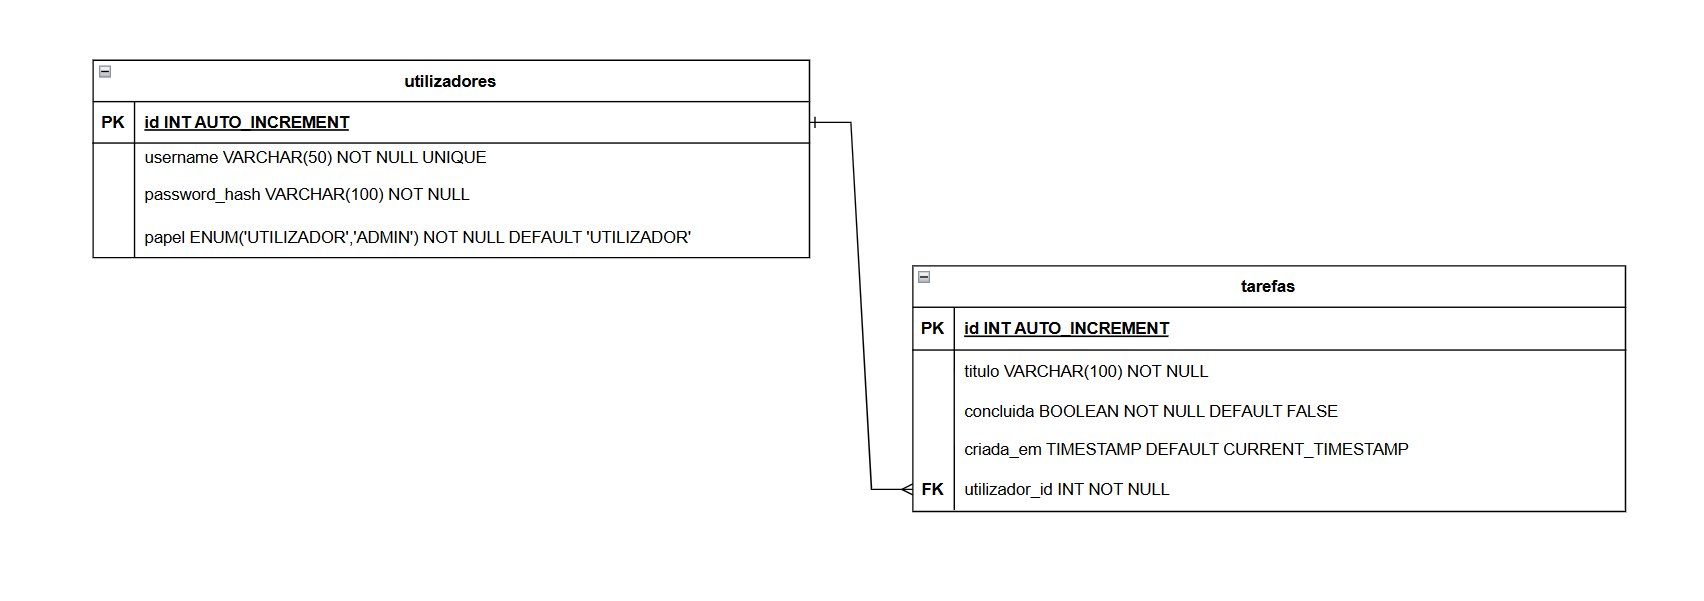
\includegraphics[scale=0.55]{figures/ModeloER.png}
  \caption{Modelo relacional simplificado das entidades \textit{Utilizador} e \textit{Tarefa}.}
	\label{fig:ermodel}
\end{figure}

\noindent Conforme ilustrado na Figura~\ref{fig:ermodel}, a entidade Utilizador armazena, entre outros campos, o atributo \code{perfil}, que distingue os registos do tipo Administrador dos registos do tipo \textit{Utilizador} comum, sendo este o campo consultado pelo \textit{back-end} para aplicar as regras de autorização descritas na Secção~\ref{sec:Ch3.2}. A entidade Tarefa inclui a chave estrangeira \code{idUtilizador}, que a associa ao seu responsável, bem como o campo \code{estado}, utilizado para representar o progresso da tarefa (por exemplo, por fazer, a fazer ou  concluída).

\section{Front-end}
\label{sec:Ch3.4}

\noindent O cliente gráfico  tem a estrutura correspondendo a cada uma a um ecrã da aplicação,  cada ecrã é associada a uma classe \textit{controller} \textit{JavaFX}, As respostas recebidas em \ac{json} são convertidas para objetos \textit{Java} antes de serem apresentadas.

\begin{itemize}
	\item \textbf{Autenticação:}~ecrã inicial onde o utilizador introduz as suas credenciais, submetidas ao \textit{endpoint} de autenticação do \textit{back-end};
	\item \textbf{Lista de Tarefas:}~apresenta, numa \code{TableView}, as tarefas do Utilizador autenticado ou, no caso do Administrador, a totalidade das tarefas registadas no sistema;
	\item \textbf{Formulário de Tarefa:}~permite a criação e a edição de uma tarefa, sendo reutilizado tanto para o Administrador como para o Utilizador;
	\item \textbf{Gestão de Utilizadores:}~ecrã exclusivo do Administrador, que lista os utilizadores registados e permite a sua criação e remoção.
\end{itemize}

A interface gráfica foi desenhada para adaptar as funcionalidades disponíveis ao perfil de acesso autenticado. Na Figura~\ref{fig:admin_view} apresenta-se a vista do utilizador com perfil de Administrador, destacando o acesso concorrente à gestão de tarefas e ao controlo de contas de utilizadores.


\begin{figure}[htbp]
    \centering
    \includegraphics[width=0.90\textwidth]{Gestao_tarefas-admin_view.png}
    \caption{Interface principal do sistema na perspetiva do perfil Administrador.}
    \label{fig:admin_view}
\end{figure}


Para além do desenho estético, a interface de autenticação contempla o tratamento imediato de erros de entrada de dados, alertando o utilizador em tempo real caso tente submeter o formulário sem preencher os campos obrigatórios (Figura~\ref{fig:login_validacao}).



\begin{figure}[htbp]
    \centering
    \includegraphics[width=0.45\textwidth]{Login.png}
    \caption{Ecrã de autenticação exibindo validação de campos obrigatórios.}
    \label{fig:login_validacao}
\end{figure}

A aplicação foi disponibilizada através de um servidor de aplicações Apache Tomcat, permitindo o acesso via navegador web. Na Figura~\ref{fig:web_admin_tarefas} é apresentada a interface Web acedida por uma conta de administrador, evidenciando as funcionalidades de gestão centralizada de todas as tarefas da plataforma, bem como o módulo de gestão e criação de novos utilizadores com diferentes níveis de privilégios.

\begin{figure}[htbp]
    \centering
    \includegraphics[width=0.90\textwidth]{tarefaslocalhost.png}
    \caption{Interface Web da aplicação em execução no Apache Tomcat (vista Administrador).}
    \label{fig:web_admin_tarefas}
\end{figure}

Em conformidade com as permissões atribuídas a cada conta, a interface Web adapta os elementos visíveis de acordo com o papel do utilizador autenticado. A Figura~\ref{fig:web_user_tarefas} ilustra a perspetiva de um utilizador comum (\texttt{eduardo}), demonstrando a restrição de acesso: este visualiza apenas as tarefas sob a sua responsabilidade e não dispõe de privilégios para apagar tarefas nem para aceder ao módulo de gestão de utilizadores.

\begin{figure}[htbp]
    \centering
    \includegraphics[width=0.50\textwidth]{eduardolocalhost.png}
    \caption{Interface Web no Apache Tomcat na perspetiva de um utilizador comum.}
    \label{fig:web_user_tarefas}
\end{figure}

\section{Back-end}
\label{sec:Ch3.5}

\noindent O \textit{back-end} é implementado como um conjunto de \textit{servlets} integrados dentro do \textit{Apache Tomcat}, organizados segundo o padrão \ac{dao} para o acesso aos dados, isolando as operações \ac{crud} sobre as entidades Utilizador e Tarefa da restante lógica de  \textit{front-end}. A Tabela~\ref{tab:endpoints} resume os principais \textit{endpoints} disponibilizados pela \ac{api} \ac{rest}.



\begin{table}[htb]
	\caption{\textit{Endpoints} da \ac{api} \ac{rest} do \textit{back-end}.}
	\label{tab:endpoints}
	\centering
	\begin{tabular}{l l l}
	\toprule
	\tabhead{Método} & \tabhead{Recurso} & \tabhead{Acesso} \\
	\midrule
		\code{POST} & \code{/auth/login} & Administrador \& Utilizador \\
		\code{GET} & \code{/tarefas} & Administrador (todas) \,/\, Utilizador (próprias) \\
		\code{POST} & \code{/tarefas} & Administrador \& Utilizador \\
		\code{PUT} & \code{/tarefas/\{id\}} & Administrador (todas) \,/\, Utilizador (próprias) \\
		\code{DELETE} & \code{/tarefas/\{id\}} & Administrador \\
		\code{GET} & \code{/utilizadores} & Administrador \\
		\code{POST} & \code{/utilizadores} & Administrador \\
		\code{DELETE} & \code{/utilizadores/\{id\}} & Administrador \\
	\bottomrule
	\end{tabular}
\end{table}

\noindent No âmbito da segurança e do princípio do menor privilégio, a ligação da base de dados é efetuada por uma conta de serviço dedicada, com acessos estritamente delimitados às tabelas necessárias (Figura~\ref{fig:db_utilizadores_privilegios}).

\begin{figure}[htbp]
    \centering
    \includegraphics[width=0.90\textwidth]{basedados_criar_utilizadores_privilegios.png}
    \caption{Configuração de privilégios de acesso e registos da tabela de utilizadores no MySQL Workbench.}
    \label{fig:db_utilizadores_privilegios}
\end{figure}

De forma a assegurar a modularidade e a clara separação de responsabilidades na camada de suporte ao servidor, o diretório de implementação organiza-se numa estrutura hierárquica bem delineada. Na Figura~\ref{fig:arvore_backend} apresenta-se a disposição dos diretórios principais.
\begin{figure}[htbp]
    \centering
    \includegraphics[width=0.75\textwidth]{tree_backend.png}
    \caption{Estrutura de pastas da aplicação evidenciando o módulo de suporte ao servidor Tomcat.}
    \label{fig:arvore_backend}
\end{figure}

\section{Sumário}
\label{sec:Ch3.6}

\noindent Neste capítulo descreveu-se a solução implementada para a aplicação \textit{Gestão de Tarefas}, assente numa arquitetura distribuída de três camadas que recorre ao \textit{JavaFX} na apresentação, ao \textit{Tomcat} na lógica de servidor e ao \textit{MySQL} na persistência de base de dados. As  camadas assim comunicam entre si por \ac{http}/\ac{json} e \ac{jdbc}, respetivamente.

